\documentclass[10pt, compress]{beamer}

\usetheme{m}

\usepackage{booktabs}
\usepackage[scale=2]{ccicons}
\usepackage{minted}

\usemintedstyle{trac}

\title{Connecting APIs for smart cities: CityBikes}
\subtitle{}
\date{\today}
\author{Gerard Casas Saez}
\institute{Universitat Politècnica de Catalunya}

\setbeamertemplate{footline}[text line]{%
  \parbox{\linewidth}{\vspace*{-8pt}\hfill\insertshortauthor\hfill\insertpagenumber}}

\begin{document}

\maketitle
\begin{frame}{Index}
\large
    \begin{itemize}
        \item Overview: What?
        \item Features - Demo
        \item Summary
    \end{itemize}
\end{frame}
\section{What?}
\begin{frame}{Goal}
\Large Help \alert{citizens} use bikes systems around the world by providing an \alert{unified platform} to find routes and read live information

\end{frame}

\begin{frame}[fragile]
\frametitle{Features}
    \large
    \begin{itemize}
        \item Show \alert{bike systems} and their station status
        \item Creates  \alert{routes for bike} in the city with optimization depending on live bike availability
        \item \alert{Route download} in different coordinate systems and different formats
  \end{itemize}
\end{frame}

\begin{frame}{Technologies}
    \begin{description}
        \item[FME Server] Automatically processes live data and runs FME Workspaces
        \item[FME Desktop] FME Workspace creation. Merges data and gives results to client.
        \item[OpenLayer] Displays Open Street Bikes Map and manages KML layers.
        \item[GoogleMaps API] Display map for Google Maps and geocodes Places into pair of coordinates
        \item[CityBikes API] Retrieves data from bike systems around the world and serves the data in a single REST API
        \item[Overpass API]  Streets data from Open Street Maps
    \end{description}
\end{frame}

\section{Bike systems}
\begin{frame}{How?}
    
    APIs:
    \begin{itemize}
        \item CityBikes - \url{citybik.es}
    \end{itemize}
    FME Workspace:
    \begin{itemize}
        \item Retrieves data from API
        \item Conversion to KML
    \end{itemize}
    
\end{frame}


\begin{frame}{Cities included}
    \begin{columns}[onlytextwidth]
        \column{0.5\textwidth}
        \begin{itemize}
            \item Barcelona
            \item London
            \item Köln
            \item Berlin
            \item Paris
        \end{itemize}
        \column{0.5\textwidth}
        \begin{itemize}
            \item Bruxelles
            \item Santander
            \item Indianapolis, IN
            \item Chicago, IL
            \item and more ...
        \end{itemize}
    \end{columns}
    
\end{frame}


% \plain{Bike Systems}{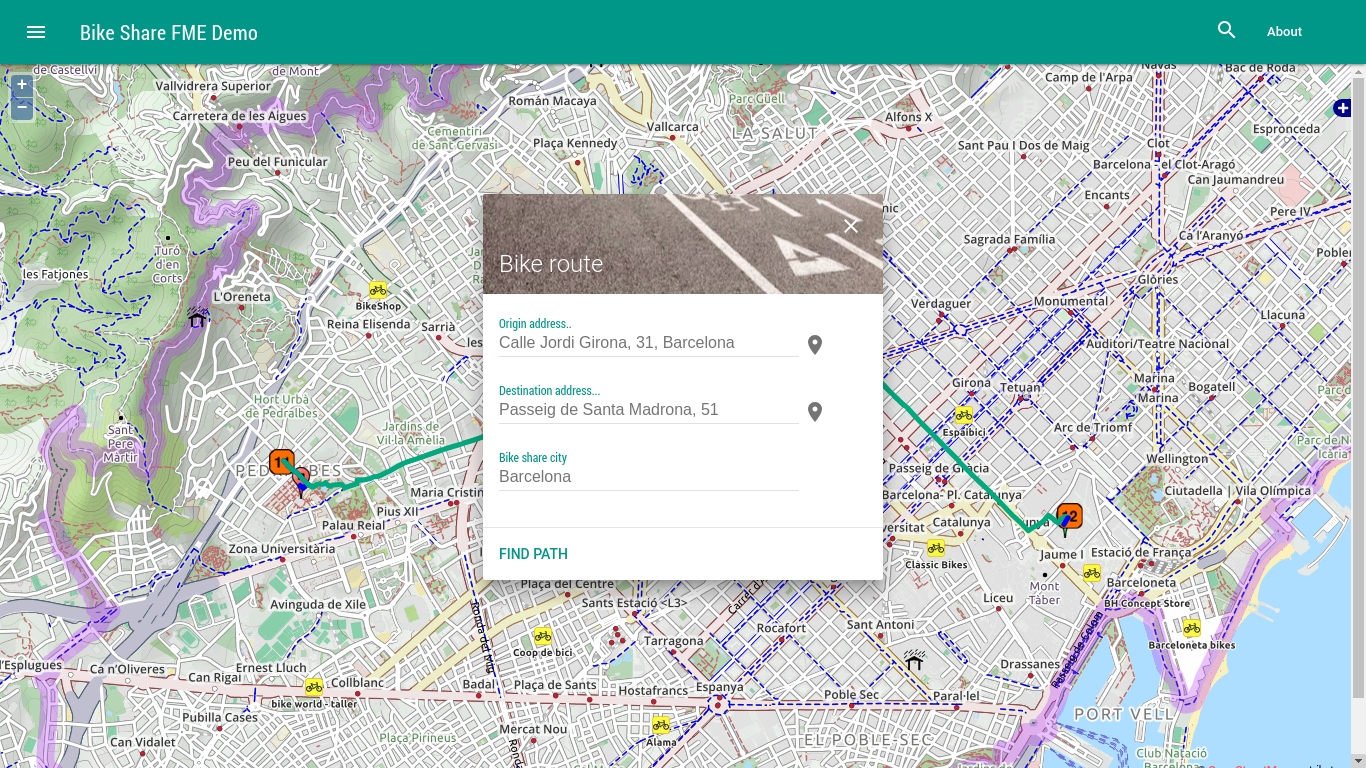
\includegraphics[width=\textwidth]{images/bike_route.png}}
{
\usebackgroundtemplate{
\vbox to \paperheight{\vfil\hbox to \paperwidth{\hfil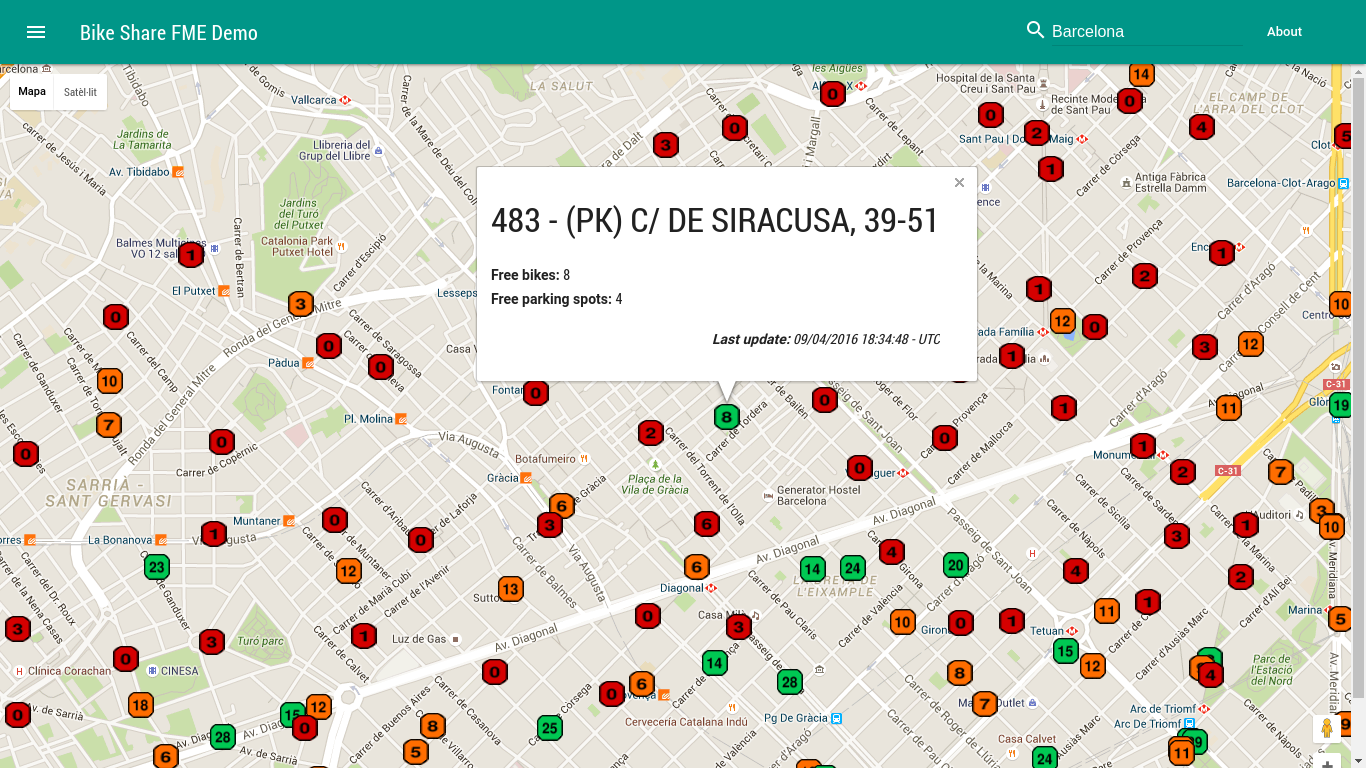
\includegraphics[height=\paperheight]{images/bikes_barcelona.png}\hfil}\vfil}
}
\plain{}{}
}

{
\usebackgroundtemplate{
\vbox to \paperheight{\vfil\hbox to \paperwidth{\hfil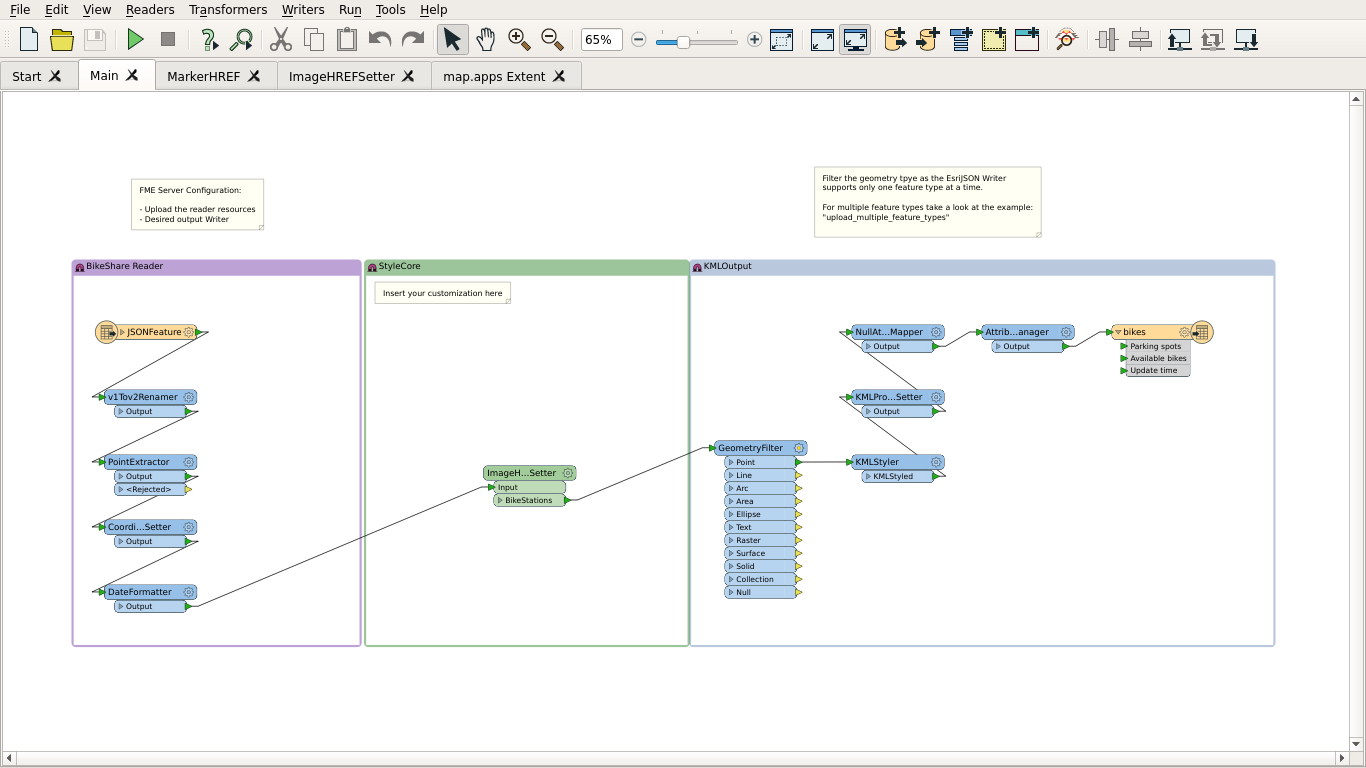
\includegraphics[width=\paperwidth]{images/workspace_bikes.png}\hfil}\vfil}
}
\plain{}{}
}

\section{Bike routing}

\begin{frame}{How?}
    
    APIs:
    \begin{itemize}
        \item CityBikes - \url{citybik.es}
        \item Overpass OSM API \url{overpass-api.de}
        \item Geocoder Google Maps API
        
    \end{itemize}
    FME Workspace:
    \begin{itemize}
        \item Custom route engine
        \item Retrieves live data from API
        \item Handles street network data from Open Street Maps
    \end{itemize}

    
\end{frame}

{
\usebackgroundtemplate{
\vbox to \paperheight{\vfil\hbox to \paperwidth{\hfil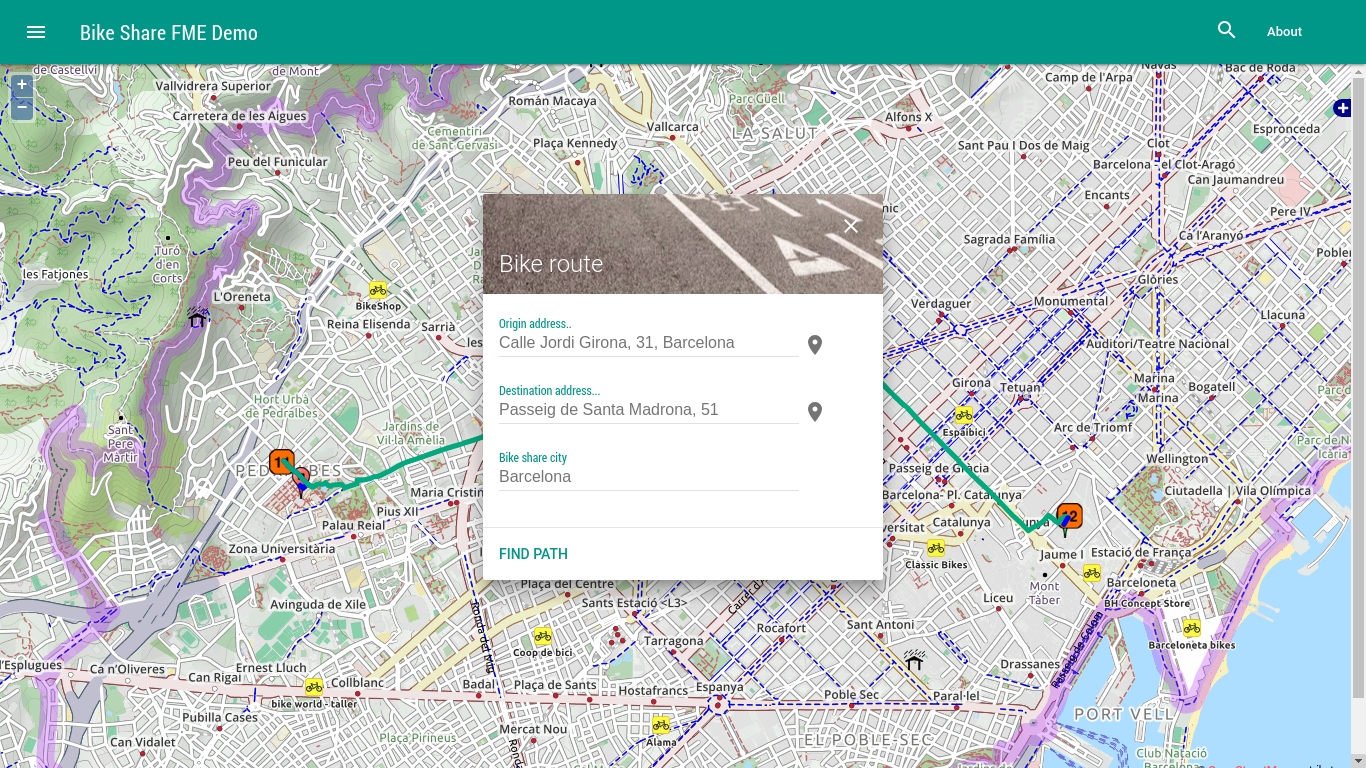
\includegraphics[height=\paperheight]{images/bike_route.png}\hfil}\vfil}
}
\plain{}{}
}

{
\usebackgroundtemplate{
\vbox to \paperheight{\vfil\hbox to \paperwidth{\hfil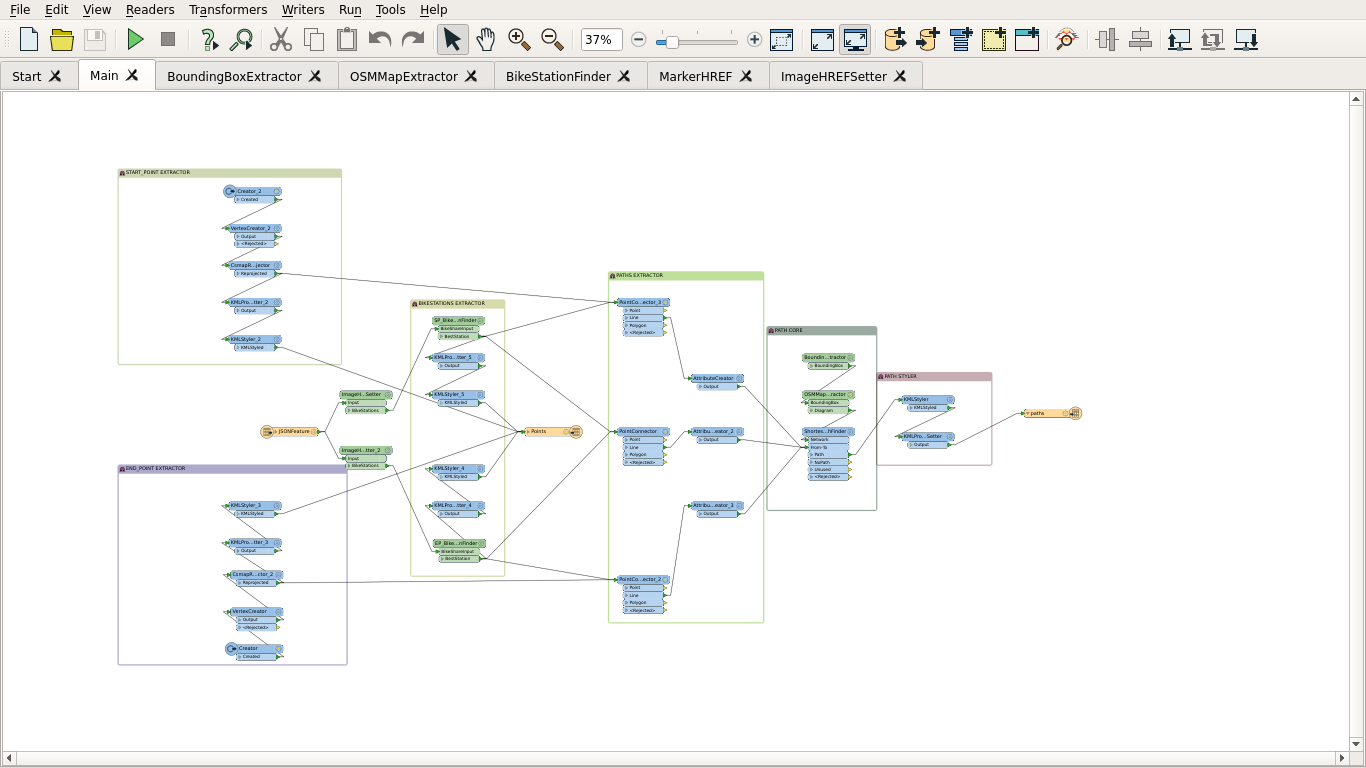
\includegraphics[width=\paperwidth]{images/workspace_path.png}\hfil}\vfil}
}
\plain{}{}
}

% \plain{Bike Routes}{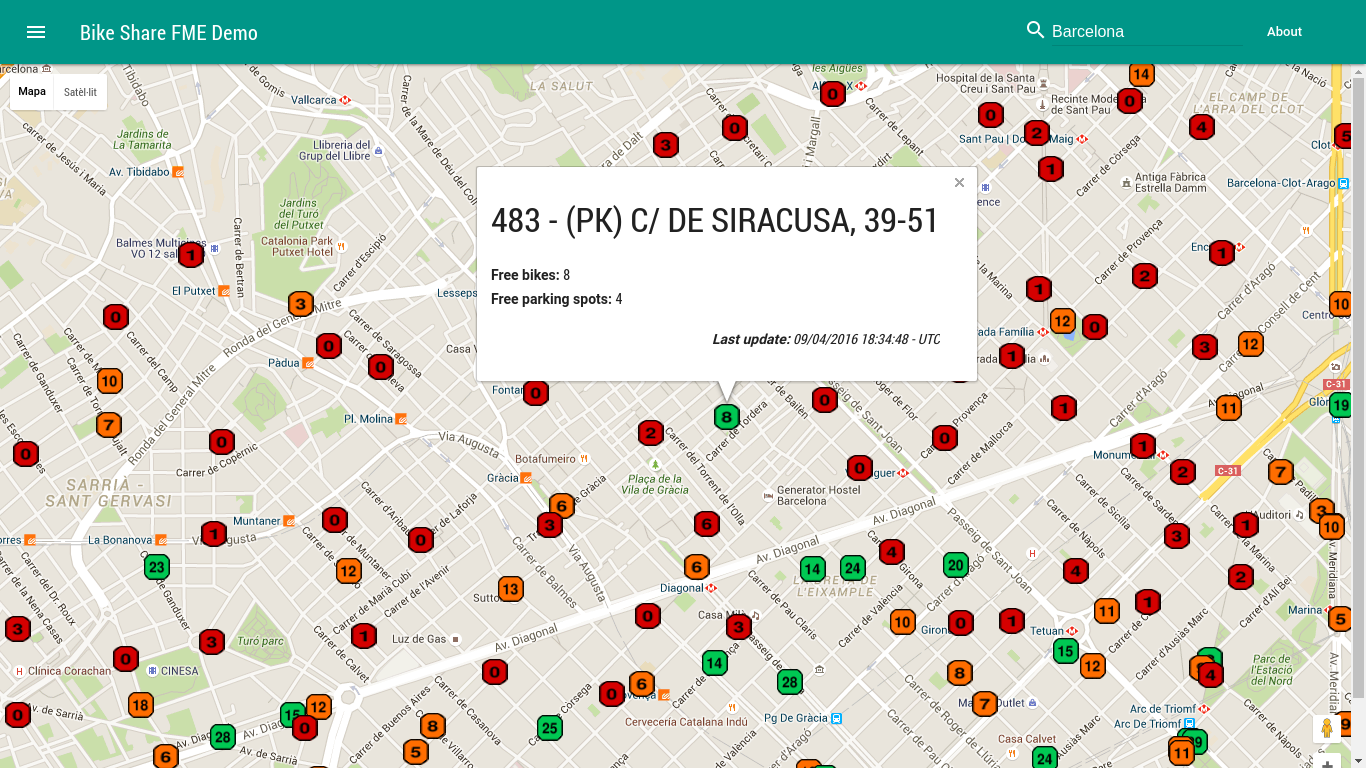
\includegraphics[width=\textwidth]{images/bikes_barcelona.png}}

\section{Route download}
\begin{frame}{How?}
    FME Workspace:
    \begin{itemize}
        \item Format conversion from KML
        \item Coordinate system conversion
    \end{itemize}
    
\end{frame}
\begin{frame}{Format}
\begin{columns}[onlytextwidth]
    \column{0.5\textwidth}
        Output formats:
        \begin{itemize}
            \item Google Earth KML
            \item GPS eXchange Format
            \item ESRI Shape
        \end{itemize}
    \column{0.5\textwidth}
        Coordinates systems
        \begin{itemize}
            \item Spherical Mercator
            \item LL-WGS84
            \item ETRS89-LCC
            \item ED50-UTM31
            \item ETRS89-UTM31N
        \end{itemize}
    \end{columns}
\end{frame}

{
\usebackgroundtemplate{
\vbox to \paperheight{\vfil\hbox to \paperwidth{\hfil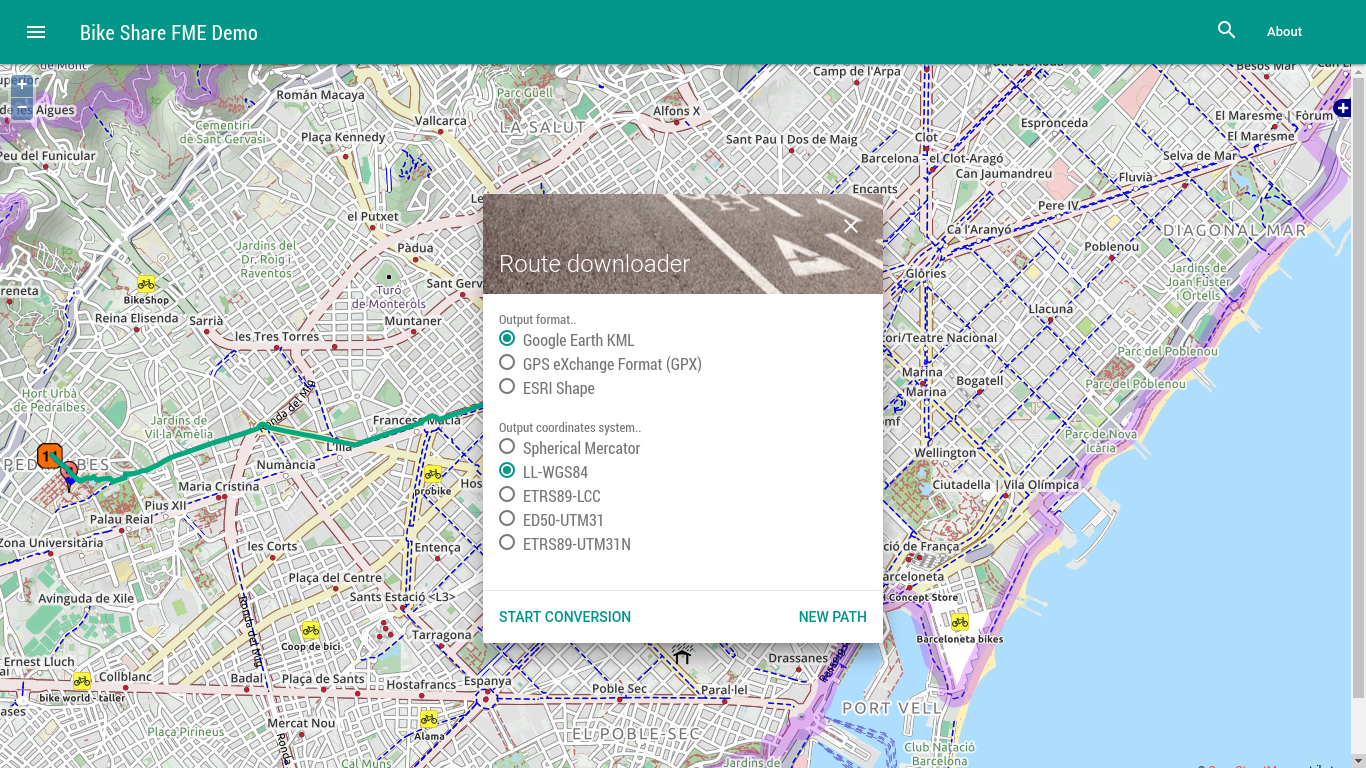
\includegraphics[height=\paperheight]{images/route_download.png}\hfil}\vfil}
}
\begin{frame}[plain]
\end{frame}
}



\section{Summary}

\begin{frame}{Summary}
    Maps
    \begin{itemize}
        \item Google Maps
        \item Open Street Maps
    \end{itemize}
    Bike stations open data
    \begin{itemize}
        \item Citybik.es
    \end{itemize}
    Streets network
    \begin{itemize}
        \item Overpass API (OSM data)
    \end{itemize}
    FME usage
    \begin{itemize}
        \item Format conversion
        \item Custom routing engine
        \item Coordinate system unificator.
    \end{itemize}

\end{frame}

\begin{frame}{Live demo}
  \begin{center}

    
\includegraphics[width=0.3\textwidth]{images/qr.png}\\
      \href{http://fmeconnect.s3-website.eu-central-1.amazonaws.com}{\url{goo.gl/oCaxJh}}
  \end{center}

  

\end{frame}

\plain{}{Questions?}



\begin{frame}
    \huge Thanks for listening! :D \\
    
    \normalsize
  \begin{description}
   \item[Name] Gerard Casas Saez
    \item[E-mail] casassg@gmail.com
    \item[Web] \href{casassg.github.io}{casassg.github.io}
    \item[Twitter] \href{twitter.com/casassaez}{@casassaez}
  \end{description}
\end{frame}

\end{document}
